\section{SINH Hyperbolic Sine Function}

\subsection{Usage}

Computes the hyperbolic sine of the argument.
The syntax for its use is
\begin{verbatim}
   y = sinh(x)
\end{verbatim}
\subsection{Function Internals}

The \verb|sinh| function is computed from the formula
\[
   \sinh(x) = \frac{e^x-e^{-x}}{2}
\]
\subsection{Examples}

Here is a simple plot of the hyperbolic sine function
@>


\centerline{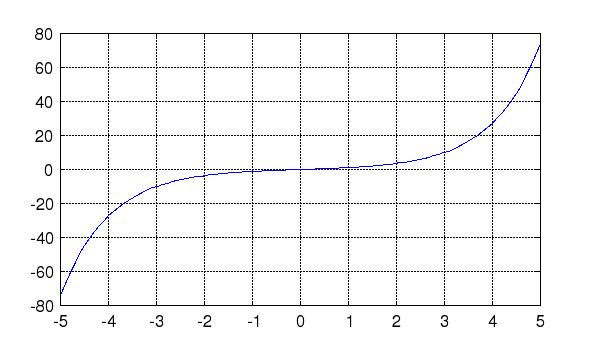
\includegraphics[width=8cm]{sinhplot}}

